\documentclass[twoside,11pt]{article}

% Any additional packages needed should be included after jmlr2e.
% Note that jmlr2e.sty includes epsfig, amssymb, natbib and graphicx,
% and defines many common macros, such as 'proof' and 'example'.
%
% It also sets the bibliographystyle to plainnat; for more information on
% natbib citation styles, see the natbib documentation, a copy of which
% is archived at http://www.jmlr.org/format/natbib.pdf

\usepackage{jmlr2e}
%\usepackage{parskip}
\usepackage{cleveref}
\usepackage{tabularx}
\newcolumntype{C}[1]{>{\centering\arraybackslash}p{#1}}

% Definitions of handy macros can go here
\newcommand{\dataset}{{\cal D}}
\newcommand{\fracpartial}[2]{\frac{\partial #1}{\partial  #2}}
% Heading arguments are {volume}{year}{pages}{submitted}{published}{author-full-names}

% Short headings should be running head and authors last names
\ShortHeadings{Predicting Taxi Revenues in Chicago}{Mitre, Su, Wild}
\firstpageno{1}

\begin{document}

\title{Developing a Predictive Model for Taxi Revenues in Chicago}

\author{\name David Mitre Becerril \email dmitrebe@andrew.cmu.edu\\
        \name Na Su \email nsu1@andrw.cmu.edu\\
        \name Raphael Wild \email rwild@andrew.cmu.edu\\
       \addr Heinz College of Information Systems and Public Policy\\
       Carnegie Mellon University\\
       Pittsburgh, PA, United States}

\maketitle

\begin{abstract}
  The taxi business has been established for many years. However, competition is becoming harder due to ridesharing services entering the market, which is why the optimization of processes is crucial for taxi companies. By this point, several analyses have been conducted with the goal of developing predictive models for the taxi business. This work presents a new way of analyzing revenues by training machine learning models to evaluate whole driving strategies instead of single trips. Trip recordings from Chicago in past years are combined into weekly statistics about each taxi. The results of this work show that machine learning models, especially random forests, are appropriate to give accurate predictions for this task.
\end{abstract}

\section{Introduction}

The taxi business in Chicago generates more than \$400 million yearly from more than 27 million rides \citep{rates}. Due to the rise of online and peer-to-peer ridesharing platforms, taxi drivers are facing more and more competition. Therefore, they need better strategies to increase their revenues. However, achieving such a goal is not an easy task given the many dynamic factors involved. To leverage the use of machine learning for taxi drivers, we built a predictive model to recommend which strategies could help taxi drivers achieve their revenue goals by predicting revenue for the trips planned in a week. For this purpose, weekly trip data for each driver is analyzed, taking into consideration the effect of how trips are distributed over time and different pickup locations as well as of other factors such as weather conditions.

\section{Background} \label{background}

Different cities have published data about taxi trips, which usually contain geo-referenced, timestamp information, along with fare costs, distance, and travel times for each trip. The granularity of the data allows making useful predictions for businesses. Previous analyses have been conducted in  Portugal \citep{TaxiTravelTime}, China \citep{TaxiDemand2}, and the US \citep{NYCTaxi}. Our project will contribute to existing work by building a machine learning model that will predict the drivers’ revenue allowing to distinguish the best behavior they could follow to increase profits.\par

The City of Chicago regularizes taxicab rates \citep{rates}. Therefore, the goal of our analysis is not to estimate dynamic rates as it might be relevant for ridesharing services like Uber \citep{uber}. Taxi fares in Chicago are mostly depending on distance, duration, and number of passengers. Additional fees may apply in case of trips starting at the airport or in form of a "Vomit Clean-up Fee". Furthermore, there is a base fare that is added to every trip. Fixed rates for certain routes are also possible.\par

\section{Methods} \label{experiment}

Before the actual analysis, the published raw trip data needs to be adapted so that it fits the idea of evaluating weekly strategies. Hence, the pre-processed data needs to be in the form of a table whose rows represent the strategy for unique combinations of taxis and weeks.\footnote{The code used for this project is publicly available at https://github.com/rwild-cmu/appliedanalytics-chicagocab} 

\subsection{Source Data}

This analysis is based on taxi trips recorded by the City of Chicago.\footnote{Link to dataset: https://data.cityofchicago.org/Transportation/Taxi-Trips/wrvz-psew/data} According to the \citet{dataDesc}, this dataset is believed to contain most of the taxi trips in the city and covers more than 100 million trips from 2013 to 2017. Each record represents one trip and includes information regarding payment, location, duration, time, distance, and the taxi company. Some records, which were suspected to be faulty (considering duration, distance, and costs), were removed by the providers of the dataset. For this work, only data from the years 2016 and 2017 was used to provide a basis for the analysis that is as recent as possible. The raw data consists of 9,122,704 trips (2016 and 2017). Unfortunately, the data for 2017 is incomplete as just the first half of the year is represented in the dataset. However, widely varying combinations are covered in the 2017 data so that it is sufficient to serve as a test set for the models introduced later.\par

The taxi trips data was supplemented with weather information from the National Oceanic and Atmospheric Administration’s Local Climatological Data \citep{NOAA}. For each trip, values for precipitation and temperature to the nearest hour when the trip started, as well as the standard deviation of precipitation and temperature for the whole day were added.

\subsection{Data Aggregation} \label{sec:aggregation}

As the analysis refers to weekly statistics rather than individual trips, the dataset needed to be aggregated by taxi (i.e., by a unique Taxi ID) and week. This is done by mapping each trip into classes, for example, there is a class "Monday 12 a.m. - 6 a.m.", which refers to the time of the trip, and a class "South Side", which refers to the pickup location. For each taxi (identified by a unique ID) and each week, the number of trips per class are counted and the fares are summed up building the revenue for the week. Two different approaches were employed in this work with respect to the final form of the features.\par

 In the first approach, the result of the aggregation is the overall revenue for each week and taxi together with percentages representing the share of a certain class on the total number of trips in a week. That is, for all categories (time, location, etc.) there will be numbers giving the percentage of trips in each class, which all sum up to one. For example, the numbers stored for the number of trips in each of the 9 sides of Chicago sum up to 1, i.e., each number represents the percentage of trips started in the respective side. Furthermore, the total number of trips is stored in the record.\par

In the other approach, the aggregated result also contains the revenue for each week and taxi but includes absolute values rather than percentages. That is, the total number of trips is not stored explicitly but represented by the sum of the numbers of trips in each class per category.\par

\subsection{Missing Data}

There are 3,474,554 records in the 2016 and 2017 dataset without information about the operating company. For these records, an additional category indicating that there is no company associated was used. Records with missing data for the pickup location (Original Name: PickupCommunityArea) were treated analogously; the 64,879 records were mapped to a category that indicates that the location is unknown. There also were missing values for Taxi ID but just very few (1,585) so that they could be excluded from the analysis without significant impact, i.e., they were ignored when aggregating the data.\par

Obviously, not all taxis were used every week of the year because of renewal, vacations of the respective driver, or possible other reasons. This leads to a large number of records (2016: 107,253; 2017: 124,508) with all values being 0. These were removed because there is no gain in information from using them. Furthermore, records were removed if their revenue was 1.5 times the interquartile range above the third quartile as they are suspected to be either faulty or, at least, very uncommon and therefore not useful for making reasonable predictions.\par

\subsection{Feature Choices} 

As the goal of this work is to predict revenue based on a distribution of trips with respect to time and location, not all trip attributes provided in the source dataset can be used. The input of the models needs to be restricted to data that can be known beforehand. Assume that a driver would plan his or her trips for the upcoming week. In that case, the driver would not be able to enter the distance or duration per trip because it is not possible for the driver to control these, e.g., a passenger chooses a destination regardless of the driver's plans. Hence, features were selected based on whether they can be controlled by taxi drivers. The core idea is that the features represent a driver's strategy of how to distribute trips over the week. The categories used for the analysis are: 1) Time, 2) Pickup location, 3) Precipitation at start of trip, 4) Temperature at start of trip, 5) Standard deviation for precipitation at day of trip, 6) Standard deviation for precipitation at day of trip, and 7) Company.

Of course, drivers cannot influence the weather itself, but, since weather is dependent on time, they could adjust their strategy to weather forecasts. The classes in the Time category are 28 intervals over the week, i.e., each weekday is divided into 4 parts. For precipitation, a boolean variable indicates whether there was some precipitation at the beginning of the trip. The classes for the other weather categories are their quartiles. For the company, only the four with the most trips were included explicitly. This is to avoid overfitting due to a low number of trips for other companies. All other companies were grouped together as "Other". See the Appendix for detailed information about the categories and their classes.

\subsection{Evaluation} \label{sec:eval}

As no work could be found where revenue is analyzed with regards to the distribution of trips for a single taxi during a week, the models in this work are compared to the performance of a simple heuristic. An obvious heuristic to be applied, based on our input, is the average revenue per trip. Hence, the models developed in this work will be compared to a prediction model that simply multiplies the average revenue per trip with the total number of trips.\par

The models will be trained using the mean squared error as a loss function and their performance will be evaluated based on this metric. An important aspect for evaluation is whether the models are able to generalize so that they work well for later years. Therefore, the models are trained on the 2016 data and tested on the 2017 data. Also, the average revenue for the heuristic refers to 2016 data.

\section{Models} \label{model}

Experiments were performed with different regression models in order to identify which fits best. The first model is linear regression, which is a simple model with an easy interpretation as the influence of individual features on the outcome can be determined by looking at the coefficients in the model. Additionally, a neural network and random forest were employed because they are expected to be more precise. However, higher precision comes at costs in terms of interpretability.

\subsection{Linear Regression}

Linear regression is used to predict the outcome, revenue, on the basis of 55 predictor variables, including counting on pickup time blocks and locations as continuous variables and companies as categorical variables. Also, experiments with regularization were done. The cv.glm function from package glmnet performs 10-fold cross validation to choose the best $\lambda$ for a fixed $\alpha$, but it does not support $\alpha$-tuning. So $\alpha$ was tuned between 0 and 1 manually. When comparing their MSE with linear regression, their MSE turned out to be slightly higher. Therefore, regularization did not improve the performance and will to be considered in the results.

\subsection{Neural Network}

Various combinations of hyperparameters were tested to come up with a good configuration. For this purpose, the 2016 data was split into a training set (80\%) and a validation set (20\%) randomly. The neural network finally employed in this analysis contains three hidden layers with 64, 256, and 64 neurons. The first two layers have a sigmoid activation, while the activation function chosen for the third and the output layer are linear. To avoid overfitting, early stopping was employed, based on another 20\% split of the training set. The network was trained for 40 epochs and the optimization algorithm employed was Nesterov Adam \citep{Nadam}.

\subsection{Random Forest}

The Random Forest was tuned using five-fold cross-validation over the training set. The model was built using 100 trees, variance as the split rule, 15 as the minimum node size, and allowing to select among 30 out of the 55 available variables to possibly split at in each node. An  R package called ranger was used the to built the model.

\section{Results} \label{results}

As this work aims to provide accurate predictions in the future, an important aspect is that the predictions should be generalizable to later years. This is why all models are evaluated based on their mean squared error (MSE) when applied to inputs from the 2017 data.

\subsection{Data Characteristics}

The datasets for the two years differ in size because the data for 2017 was only recorded for the first half of the year. The aggregated data for 2016 has 169,133 rows, 2017 has 58,907 rows. Tables \ref{tab:data_characteristics1}, \ref{tab:data_characteristics2}, and \ref{tab:data_characteristics3} describe the characteristics of the data (absolute valued covariates) for the respective years. Noticeably, the data for 2017 does not only have less rows, there also were less trips per taxi and week resulting in lower revenues.

\begin{table}[H]
    \centering
    \begin{tabular}{c|c|c}
         & 2016 mean (SD) & 2017 mean (SD)\\
         \hline
        Revenue & 470.3 (204.4) & 343.0 (153.4)\\
        No rain & 31.8 (17.1) & 23.4 (13.5)\\
        Rain & 3.4 (3.8) & 3.1 (3.6)\\
        Monday night & 0.3 (1.0) & 0.2 (0.8)\\
        Monday morning & 1.1 (1.7) & 0.9 (1.4)\\
        Monday afternoon & 1.6 (1.9) & 1.3 (1.6)\\
        Monday evening & 1.4 (1.8) & 1.1 (1.5)\\
        Tuesday night & 0.2 (0.7) & 0.1 (0.5)\\
        Tuesday morning & 1.2 (1.8) & 1.0 (1.6)\\
        Tuesday afternoon & 1.8 (2.0) & 1.5 (1.7)\\
        Tuesday evening & 1.7 (2.0) & 1.3 (1.7)\\
        Wednesday night & 0.4 (1.2) & 0.2 (0.5)\\
        Wednesday morning & 1.3 (1.8) & 1.1 (1.6)\\
        Wednesday afternoon & 1.9 (2.0) & 1.6 (1.8)\\
        Wednesday evening & 1.8 (2.0) & 1.5 (1.7)\\
        Thursday night & 0.3 (0.9) & 0.2 (0.6)\\
        Thursday morning & 1.3 (1.8) & 1.1 (1.6)\\
        Thursday afternoon & 2.0 (2.0) & 1.6 (1.9)\\
        Thursday evening & 2.0 (2.1) & 1.5 (1.8)\\
        Friday night & 0.5 (1.2) & 0.2 (0.7)\\
        Friday morning & 1.2 (1.7) & 1.0 (1.5)\\
        Friday afternoon & 2.1 (2.1) & 1.7 (1.9)\\
        Friday evening & 2.2 (2.3) & 1.6 (1.9)\\
        Saturday night & 1.1 (1.9) & 0.6 (1.4)\\
        Saturday morning & 0.6 (1.2) & 0.4 (0.9)\\
        Saturday afternoon & 1.5 (1.9) & 1.0 (1.5)\\
        Saturday evening & 2.0 (2.3) & 1.3 (1.8)\\
        Sunday night & 1.3 (2.3) & 0.9 (1.8)\\
        Sunday morning & 0.5 (1.1) & 0.4 (0.8)\\
        Sunday afternoon & 1.1 (1.7) & 0.8 (1.3)\\
        Sunday evening & 1.0 (1.6) & 0.7 (1.2)
    \end{tabular}
    \caption{Data characteristics.}
    \label{tab:data_characteristics1}
\end{table}

\begin{table}[H]
    \centering
    \begin{tabular}{c|c|c}
         & 2016 mean (SD) & 2017 mean (SD) \\
         \hline
        Temperature Q1 & 7.0 (13.7) & 6.9 (9.9)\\
        Temperature Q2 & 5.0 (8.2) & 6.7 (7.3)\\
        Temperature Q3 & 5.3 (8.6) & 6.5 (7.1)\\
        Temperature Q4 & 17.9 (19.1) & 6.5 (8.7)\\
        Temperature SD Q1 & 6.1 (9.2) & 6.6 (9.1)\\
        Temperature SD Q2 & 10.5 (10.3) & 6.8 (7.4)\\
        Temperature SD Q3 & 10.6 (10.0) & 7.0 (6.7)\\
        Temperature SD Q4 & 8.0 (10.5) & 6.1 (6.8)\\
        Precipitation SD Q1 & 16.4 (12.6) & 11.0 (10.2)\\
        Precipitation SD Q2 & 2.5 (4.5) & 2.7 (3.9)\\
        Precipitation SD Q3 & 8.8 (9.8) & 6.3 (6.4)\\
        Precipitation SD Q4 & 7.4 (8.8) & 6.5 (7.3)\\
        Far North & 4.0 (3.9) & 3.1 (3.3)\\
        Northwest & 0.2 (0.7) & 0.1 (0.7)\\
        North & 3.8 (4.3) & 2.2 (2.8)\\
        West & 4.2 (4.6) & 3.1 (4.0)\\
        Central & 21.7 (14.4) & 17.2 (12.3)\\
        Southwest & 0.8 (1.7) & 0.5 (1.4)\\
        South & 0.3 (1.2) & 0.2 (0.9)\\
        Far Southwest & 0.0 (0.1) & 0.0 (0.1)\\
        Far Southeast & 0.0 (0.3) & 0.0 (0.2)\\
        Side unknown & 0.3 (1.4) & 0.1 (0.5)\\
    \end{tabular}
    \caption{Data characteristics (continued)}
    \label{tab:data_characteristics2}
\end{table}

\begin{table}[H]
    \centering
    \begin{tabular}{c|c|c}
         & 2016 no. (\%) & 2017 no. (\%) \\
         \hline
         Taxi Affiliation Services & 44,675 (26.4) & 9,669 (16.4)\\
         Dispatch Taxi Affiliation & 15,026 (8.9) & 4,086 (6.9)\\
         Blue Ribbon Taxi Association Inc.& 10,866 (6.4) & 3,780 (6.4)\\
         Choice Taxi Association & 12,687 (7.5) & 5,001 (8.5)\\
         Other & 85,879 (50.8) & 36,371 (61.7)
    \end{tabular}
    \caption{Data characteristics (continued)}
    \label{tab:data_characteristics3}
\end{table}

It is reasonable to expect that weather is correlated with taxi drivers' revenue. Figure \ref{fig:figure1} shows a negative, but weak correlation, within these two variables: when most of the weekly trips are done while it is raining, usually the revenue is not above \$700. However, it is more likely to have earnings above this threshold if there is some rain. Mainly, if one-fourth of the trips experienced rain, then a driver will more likely earned above \$700 in the week.

\begin{figure}[H]
  \begin{center}
    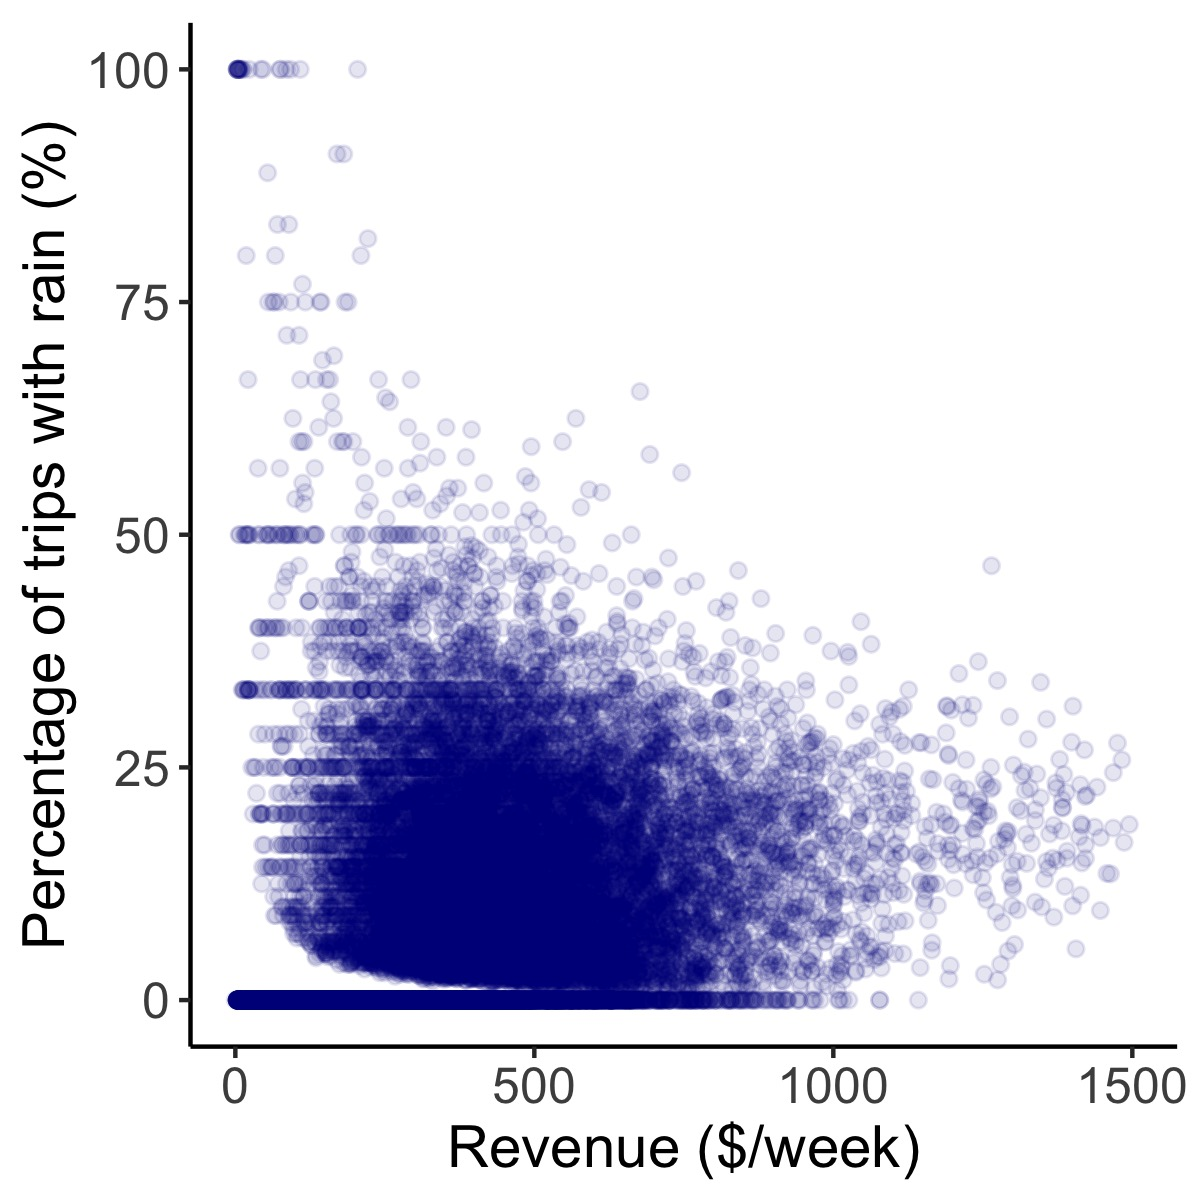
\includegraphics[height=8cm]{Plot_rainy_and_revenue.jpg}
    \caption{Correlation between revenue and rain, 2017}
    \label{fig:figure1}
  \end{center}
\end{figure}

\subsection{Performance}

\begin{table}[H]
    \centering
    \begin{tabular}{C{3cm}|C{2cm}|C{2cm}|C{2cm}|C{2cm}}
        & Linear Regression & Neural Network & Random Forest & Simple Heuristic\\
        \hline
        Test MSE (Perc) & 30,135.0 & 29,582.4 & 34,639.2 & 93,250.9\\
        Test MSE (Abs) & 5,925.0 & 5,598.2 & 5,221.9 & 93,250.9
    \end{tabular}
    \caption{Models and their mean squared error on the test set for percentages and absolute-valued features.}
    \label{tab:performance}
\end{table}

The models were analyzed with both data represented as percentages and as absolute values (see \Cref{sec:aggregation}). The two different ways of representing the same data lead to completely different results. \Cref{tab:performance} shows the average MSE for each model measured in five runs compared to the heuristic introduced in \Cref{sec:eval}.\par

For the values stored as percentages, the Random Forest gave the least accurate results (MSE 34,639). The Linear Regression was more accurate (MSE 30,135), which means that a simpler model is preferable to a Random Forest in this case. Better results were achieved with the Neural Network. On the 2017 data, the average measured loss was 29,582.4, which is by far better than the simple heuristic, but only little better than the performance of linear regression. However, the performance on the validation set that was drawn out of the 2016 data (20\% split) was by far better than the results on the 2017 test set. The MSE on the validation set was just 5856.9.\par

If the features are absolute values, performance of all models increases significantly. The Random Forest performs best (MSE 5,221.9), with the Linear Regression model showing the worst results (MSE 5,925.0), which are still by far better than for percentage inputs. The performance of the Neural Network is in between these two models (MSE 5,598.2).

Figure \ref{fig:figure2} shows the observed and the predicted revenue in 2017 using the Random Forest built using the features with absolute values. There are more values over the 45-degree line, so the predicted revenue tends to be higher than the observed one. Also, there is no single observed revenue over \$630, while there are predicted values up to \$800. 

\begin{figure}[H]
  \begin{center}
    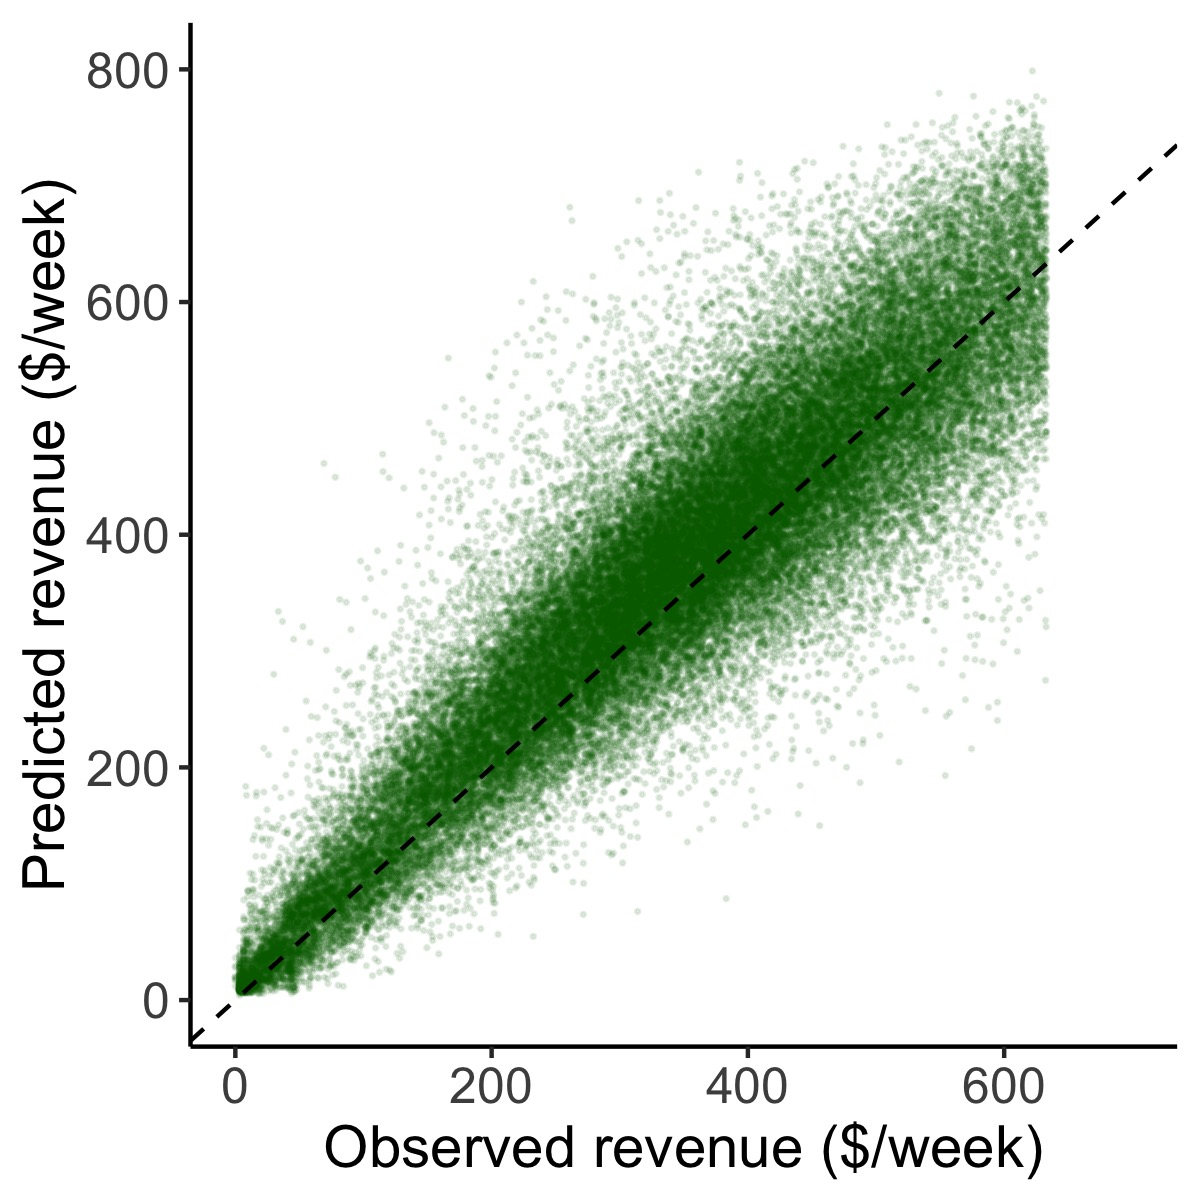
\includegraphics[height=8cm]{Plot_predicted_observed.jpg}
    \caption{Prediction vs observed revenue, 2017}
    \label{fig:figure2}
  \end{center}
\end{figure}


\subsection{Analysis of Weights}
Since the performance of the linear regression model built using absolute values outweighs the one using percentage features, and it is easy to interpretate, its coefficients are analyzed here. According to the linear regression output and coefficients' p-value, important predictors variables, that are significantly associated to the outcome variable, are some specific time blocks, temperature first quartile, different districts in Chicago and different companies, as shown in Table \ref{tab:coef_ols_abs}.

\begin{table}[h]
    \centering
    \begin{tabular}{c|c}
        Coefficient & Predictor \\ 
        \hline
        norain & 13.2518 (\****) \\
        rain & 13.6747 (***) \\
        MonNight & 0.8932 (**) \\
        MonMorning & 1.1427 (***) \\
        TueNight & 0.9868 (*) \\
        FriNight & -1.6186 (***)\\
        SatMorning & 3.4839 (***) \\
        SunMorning & 7.4614 (***) \\
        SunAfternoon & 1.7870 (***) \\
        temp0 & -0.9021 (***) \\
        Far.North & 13.8722 (***) \\
        Northwest & -6.6501 (***) \\
        North  & -6.3911 (***) \\
        West & -5.4721 (***) \\
        Central & -3.9713(***) \\
        Southwest & 17.7195 (***) \\
        South & 2.6556 (***) \\
        Far.Southwest & 5.7846 (**) \\
        Far.Southeast & 2.4286 (**) \\
        Taxi.Affiliation.services & 3.7585 (***) \\
        Dispatch.Taxi.Affiliation.Inc. & 14.4754 (***) \\
        Blue.Ribbon.Taxi.Association.Inc & -8.2808 (***) \\
        Choice.Taxi.Association & 11.4672 (***) \\
    \end{tabular}
    \caption{Coefficients for linear regression with absolute values.}
    \label{tab:coef_ols_abs}
\end{table}


\section{Discussion} 

All models came with a significant increase in performance compared to the introduced simple heuristic. Moreover, the Random Forest gives the best results when applying absolute values, which shows the benefit of more complex models. Considering their accuracy, it is likely that they can be useful for taxi companies and drivers to predict revenue and support business decision-making.\par

An interesting observation is that percentages do not work as well as absolute values for the inputs, especially because the performance on the validation set was comparable. Apparently, the models -- when trained on percentages -- fail to generalize to other years, especially the Random Forest apparently does not capture the relationships in the percentage data. However, when using absolute values, the models are generalizing well and show good results for a year that they were not trained on.\par

There are some conclusions that can be drawn from the coefficients of the Linear Model shown in Tables  \ref{tab:coefficients_perc} and \ref{tab:coefficients_perc2}. Since no rain and rain have similar coefficients, we can not conclude rainy weather would affect revenue significantly. Among all the time blocks, we can see Sunday Morning having highest coefficient. It means for every additional trip on Sunday morning, we can expect revenue to increase by average of 7.4614 dollars. For sides in Chicago, Far North and Southwest stand out. A unit increase in trips from Far North results in an increase in average revenue by 13.87 dollars, all other variables held constant. There is an international airport in Far North side so it is reasonable to make more revenue because of its large volumes and demands. But a unit increase in trips from Southwest results in a larger increase in average revenue by 17.72 dollars, all other variables held constant. Therefore, Southwest side would be another good choice to go. On the contrary, for every additional trip from Northwest, the average revenue decrease by 6.65 dollars. Also, the company that is operated for affects the revenue. In general, revenue can be expected to be higher by 14.47 dollars for trips executed by Dispatch Taxi Affiliation Inc. than those executed by other companies. 

One needs to be aware that this analysis only predicts revenues and does not consider profitability. A possible extension of this analysis would be to choose profit rather than revenue as an outcome, but this requires knowledge of costs, which cannot be obtained without expert knowledge on the application domain. The covered distance and duration of trips are included in the source data, which might be a basis for cost estimates.\par

Furthermore, the prediction models do not consider special events that may have a large impact on the taxi business such as holidays or sporting events. For example, the area around stadiums might become more profitable in case of an important game.\par

Another assumption we placed is that taxi drivers can influence time and location of their trips, which is probably true to a certain extent. However, it is not guaranteed that they will be able to pick up a passenger at the time and location they would like to, especially if multiple drivers are following the same recommendation. The problem is that the data available only contains data about trips that were actually executed but not the actual demand and supply. That is, there could be passengers in certain locations that would have wanted to take a taxi but could not get one or there could be a lot of taxis waiting at a certain location for a long time without a customer. Hence, the recommendations in this work could send a driver to a place where there is a lot of competition.

\section{Conclusion}

The taxi business generates large revenues despite the fierce competition faced from ridesharing platforms, which is why analyses in this area are important. This project shows that taxi drivers could find meaningful patterns from using a machine learning model to predict their weekly revenues. Mainly, a Random Forest suits best for this task. Future research could improve the model by increasing the feature space and tailoring the model to meet specific needs of the taxi drivers by applying expert domain knowledge.

\bibliography{websources}

\appendix
\section*{Appendix}

\Cref{tab:categories_classes} lists the classes for all categories.

\begin{table}[H]
    \centering
    \begin{tabular}{c|c}
        Category & Classes \\
        \hline
        \hline
        Time & Monday Night \textit{(12 a.m. - 6 a.m.)} \\
         & Monday Morning \textit{(6 a.m. - 12 p.m.)} \\
         & Monday Afternoon \textit{(12 p.m. - 6 p.m.)} \\
         & Monday Evening \textit{(6 p.m. - 12 a.m.)} \\
         & Tuesday Night \textit{(12 a.m. - 6 a.m.)} \\
         & ... \\
         \hline
         Pickup Location & Far North \\
         & Northwest \\
         & North \\
         & West \\
         & Central \\
         & Southwest \\
         & South \\
         & Far Southwest \\
         & Far Southeast \\
         & Unknown \\
         \hline
         Precipitation & Rain \textit{(any precipitation)} \\
         & No Rain \\
         \hline
         Temperature & \textit{By quartile} \\
         \hline
         Standard Deviation Precipitation & \textit{By quartile} \\
         \hline
         Standard Deviation Temperature & \textit{By quartile} \\
         \hline
         Company & Taxi Affiliation Services \\
         & Dispatch Taxi Affiliation \\
         & Blue Ribbon Taxi Association Inc. \\
         & Choice Taxi Association \\
         & Other
    \end{tabular}
    \caption{Feature categories and respective classes.}
    \label{tab:categories_classes}
\end{table}

\begin{table}[H]
    \centering
    \begin{tabular}{c|c}
        Coefficient & Predictor \\ 
        \hline
        \hline
        norain & 13.2518 (***) \\
        rain & 13.6747 (***) \\
        MonNight & 0.8932 (**) \\
        MonMorning & 1.1427 (***) \\
        MonAfternoon & 0.4623 (*) \\
        MonEvening & -0.1197 \\
        TueNight & 0.9868 (*) \\
        TueMorning & 0.6632 (**) \\
        TueAfternoon & -0.2295 \\
        TueEvening & -0.4699 (*) \\
        WedNight & 0.1553 \\
        WedMorning & 0.2617 \\
        WedAfternon & -0.0434 \\
        WedEvening & -0.0547 \\
        ThuNight & 0.0654 \\
        ThuMorning & 0.4533 (*) \\
        ThuAfternoon & 0.0481 \\
        ThuEvening & -0.2459 \\
        FriNight & -1.6186 (***)\\
        FriMorning & 0.2712 \\
        FriAfternoon & 0.3557 \\
        FriEvening & -0.0532 \\
        SatNight & -0.4523 (*) \\
        SatMorning & 3.4839 (***) \\
        SatAfternoon & 0.5027 (*) \\
        SatEvening & -0.3098 \\
        SunNight &  0.0854 \\
        SunMorning & 7.4614 (***) \\
        SunAfternoon & 1.7870 (***) \\
%        SunEvening & NA \\
        temp0 & -0.9021 (***) \\
        temp1 & -0.8763 (***) \\
        temp2 & 0.2597 (***) \\
%        temp3 & NA \\
        tempsd0 & -0.2110 (***) \\
        tempsd1 & -0.4008 (***) \\
        tempsd2 & -0.0242 \\
%        temp_sd3 & NA \\
        rainsd0 & 0.1352 (***) \\
        rainsd1 & -0.1584 (*) \\
        rainsd2 & 0.3667 (***) \\
%        rain_sd3 & NA \\
    \end{tabular}
    \caption{Coefficients for linear model with absolute values}
    \label{tab:coefficients_abs}
\end{table}

\begin{table}[H]
    \centering
    \begin{tabular}{c|c}
        Coefficient & Predictor \\ 
        \hline
        \hline
        Far.North & 13.8722 (***) \\
        Northwest & -6.6501 (***) \\
        North  & -6.3911 (***) \\
        West & -5.4721 (***) \\
        Central & -3.9713(***) \\
        Southwest & 17.7195 (***) \\
        South & 2.6556 (***) \\
        Far.Southwest & 5.7846 (**) \\
        Far.Southeast & 2.4286 (**) \\
%        Unknown & NA \\
        Taxi.Affiliation.services & 3.7585 (***) \\
        Dispatch.Taxi.Affiliation.Inc. & 14.4754 (***) \\
        Blue.Ribbon.Taxi.Association.Inc & -8.2808 (***) \\
        Choice.Taxi.Association & 11.4672 (***) \\
%        Other & NA \\
    \end{tabular}
    \caption{Coefficients for linear model with absolute values (continued)}
    \label{tab:coefficients_abs2}
\end{table}

\begin{table}[H]
    \centering
    \begin{tabular}{c|c}
        Coefficient & Predictor \\ 
        \hline
        \hline
        total & 10.3327 (***) \\
        rain & 14.7229 (***) \\
        MonNight & -8.7575 \\
        MonMorning & 5.7481 \\
        MonAfternoon & -4.1627 \\
        MonEvening & -5.9887 \\
        TueNight & 14.9076 \\
        TueMorning & 41.0693 (***) \\
        TueAfternoon & 11.1272 (*)\\
        TueEvening & 3.6802 \\
        WedNight & 17.5353 \\
        WedMorning & 39.7761 (***) \\
        WedAfternon & 17.8364 (***) \\
        WedEvening & 21.1507 (***) \\
        ThuNight & 24.5679 (*) \\
        ThuMorning & 57.1806 (***) \\
        ThuAfternoon & 19.3795 (***) \\
        ThuEvening & 8.2308 \\
        FriNight & 2.0758\\
        FriMorning & 40.5258 (***) \\
        FriAfternoon & 40.9495 (***) \\
        FriEvening & 11.5053 (*) \\
        SatNight & -1.6745 \\
        SatMorning & 126.7823 (***) \\
        SatAfternoon & 56.7011 (***) \\
        SatEvening & 18.6568 (**) \\
        SunNight &  4.9564 \\
        SunMorning & 126.6553 (***) \\
        SunAfternoon & 37.8195 (***) \\
%        SunEvening & NA \\
        temp1 & 4.6482 (**) \\
        temp2 & 54.0259 (***) \\
        temp3 & 43.8121 (***) \\
        tempsd1 & -9.4850 (***) \\
        tempsd2 & 1.4703 \\
        tempsd3 & 21.5288 (***) \\
        rainsd1 & -29.2635 (***) \\
        rainsd2 & 23.3935 (***) \\
        rainsd3 & 5.8990 (***) \\
    \end{tabular}
    \caption{Coefficients for linear model with percentage values}
    \label{tab:coefficients_perc}
\end{table}

\begin{table}[H]
    \centering
    \begin{tabular}{c|c}
        Coefficient & Predictor \\ 
        \hline
        \hline
        Far.North & 279.9477 (***) \\
        Northwest & -65.2082 (***) \\
        North  & -78.9868 (***) \\
        West & -80.8081 (***) \\
        Central & -13.4564 (***) \\
        Southwest & 245.8660 (***) \\
        South & 10.2127 (*) \\
        Far.Southwest & 78.0627 (**) \\
        Far.Southeast & 5.5589 \\
%        Unknown & NA \\
        Taxi.Affiliation.services & 19.3681 (***) \\
        Dispatch.Taxi.Affiliation.Inc. & 17.5472 (***) \\
        Blue.Ribbon.Taxi.Association.Inc & -1.4325 \\
        Choice.Taxi.Association & 24.5546 (***) \\
%        Other & NA \\
    \end{tabular}
    \caption{Coefficients for linear model with percentage values (continued)}
    \label{tab:coefficients_perc2}
\end{table}


\end{document}
